\refstepcounter{PagePtr}\label{P:HP}
\refstepcounter{Exercise}
\subsection*{2−2 \theExercise 自分のホームページを公開しよう\label{E:myHP}}
% \subsection*{2−2自分のホームページを公開しよう}
考え方


クライアントとサーバーと呼ばれるコンピュータがあります。クライアントとはサービスを利用するコンピュータです。サーバーとはそれと\ruby{逆}{ぎゃく}にサービスを提供しているコンピュータです。クライアントとサーバーは同じコンピュータにあっても
OK です。例えば、Googleは検索するためのウェブサイトを提供しています。ウェブサイトを提供するサーバーをウェブサーバーと呼びます。自分のホームページを公開するためには、ウェブサーバーを動かす必要があります。

注意

今回のみんなのホームページはローカルIPの間だけです。つまり、インターネット上に公開はしません。これを公開して、実際確認したりみんなで見せ合いをしてみましょう。


\bigskip

1.まず
{\textasciitilde}/07/wwwのディレクトリに移りましょう。

\ \ ターミナルを立ち上げて次のコマンドを打ちましょう。

\ \ cd {\textasciitilde}/07/www


\bigskip

2.サーバーを動かしてみましょう。

\ \ 次のコマンドを打ちましょう。

\ \  ./webserver.py

\ \ を実行するとウェブサーバが動き始めます。

\ \ webserver.pyを起動したディレクトリがドキュメントルートになります。

\ \ これはファイルシステムのルートディレクトリとは別のものでドキュメントルートはウェブ

\ \ サーバから見たルートディレクトリのことです。

\ \ つまりウェブサーバーしかそのディレクトリをルートディレクトリとは認識しません。

\ \ ディレクトリに関しては第3回の教科書3.3.2 「ディレクトリの関係」を参考にしてください。


\centering
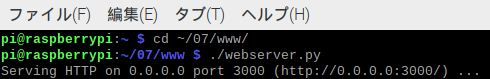
\includegraphics[width=0.73\textwidth]{text07-img/ome7-img038.png}
\flushleft

3.サーバーが動いているかどうかを確認してみましょう。

\ \ 別のターミナルを立ち上げ、次のコマンドを打ちましょう。

\ \  nmap localhost

\ \ 今回使っているポート番号は:3000です。STATE(状態)がopen(開く)になっています。

\ \ これでサーバーが動いていることが分かります。

\centering
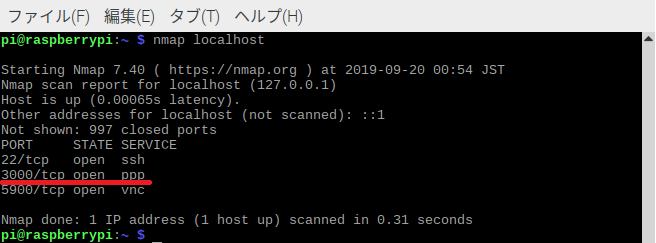
\includegraphics[width=0.75\textwidth]{text07-img/ome7-img039.png}
\flushleft

\clearpage


4.みなさんが作ったウェブページを表示してみましょう。

\ \ みなさんが作ったindex.htmlの場所はwebserver.pyを起動したディレクトリと同じでしたね。「2」で説明したドキュメントルートです。

\ \ これはwebserver.pyを起動したディレクトリ

\ \  {\textasciitilde}/07/www/

\ \ を指しています。


\bigskip

\ \ 次にブラウザのアドレスバーに打つURLはどのように書けばいいのでしょうか。

\ \ URLの書き方は次のようになります。

\ \ なので自分のパソコンのサーバーを見るには

\centering

\includegraphics[width=13.894cm]{text07-img/ome7-img040.png}
\flushleft

\ \  \url{http://localhost:3000/}

\ \ というURLになります。

\ \ サーバー名の後の/(スラッシュ)はドキュメントルートを示しています。

\ \ サーバはファイル名を指定しないとindex.htmlというファイルを開くように\ruby{設定}{せってい}されて\ \ います。

\ \  \url{http://localhost:3000/}

\ \ をブラウザのアドレスバーに打ってみましょう。

\ \ みなさんが作ったウェブページのHTMLが表示されましたね。

\ \ これは

\ \  \url{http://localhost:3000/index.html}

\ \ と入力しているのと同じことです。

\bigskip

\centering
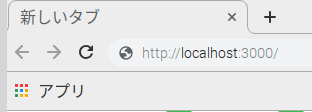
\includegraphics[width=9.551cm]{text07-img/ome7-img041.png}
\flushleft


\bigskip


\bigskip